\chapter{Exercícios}


\section{1º/2017}
\begin{exercicio}
  {2º/2017}{\textit{Threads}}
  {Por quê a implementação de \textit{threads} em nível de usuário possui um custo extremamente baixo de troca de contexto?}

  Comparando o custo da troca de contexto à nível de kernel com a implementação à nível \textit{threads}, o custo é extremamente baixo pois as trocas de contexto entre \textit{threads} não possuem o custo da troca de modo usuário para protegido, uma vez que esta troca é feita em nível de aplicação, existindo apenas no nível de usuário. À nível de \textit{threads} se resume a utilizar conjunto de instruções de \textit{load}, \textit{store} e \textit{jump} para simular uma troca de contexto, enquanto à nível kernel alterna entre modo usuário para protegido e modo usuário utilizando-se instruções de \textit{long jump}.
\end{exercicio}

\begin{exercicio}
  {2º/2017}{Condições de Corrida}
  {Defina condição de corrida. Considere o código multi-processo abaixo. Existe condição de corrida nesse código? Se sim, corrija o código de maneira a eliminá-la.
  \begin{figure}[H]
    \centering
    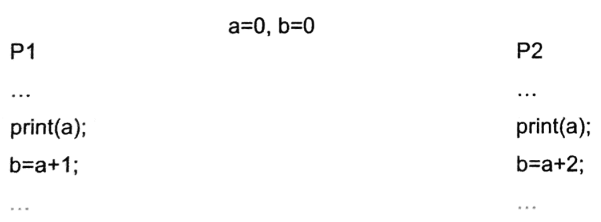
\includegraphics[width=0.5\textwidth]{ex-race-cond}
  \end{figure}}

  \textbf{Condição de Corrida:} quando dois ou mais processos acessam concorrentemente um recurso e o resultado final sobre este recurso depende da ordem na qual os processos foram executados.

  Sim, existe condição de corrida na variável $b$. Utilizamos \textit{locks} para a nossa solução:

  \begin{table}[H]
    \centering
    \begin{tabular}{l|l}
      \textbf{P1:}            & \textbf{P2:} \\
      \texttt{print(a)}       & \texttt{print(a)} \\
      \texttt{acquire(lock)}  & \texttt{acquire(lock)} \\
      \texttt{b = a + 1}      & \texttt{b = a + 2} \\
      \texttt{release(lock)}  & \texttt{release(lock)}\\
    \end{tabular}
  \end{table}
\end{exercicio}

\begin{exercicio}
  {2º/2017}{\textit{Deadlocks}}
  {Por quê \textit{deadlocks} são ditos \textit{stable properties}?}

  Pois consistem em estados que não podem ser mudados sem utilização de força externa.
\end{exercicio}

\begin{exercicio}
  {2º/2017}{Arquivos}
  {Qual a função da operação \texttt{OPEN} e \texttt{CLOSE}?}

  \texttt{OPEN:} fazer a associação entre o processo e o arquivo, através da tabela de descritores, retornando um descritor que será usado nas próximas operações.

  \texttt{CLOSE}: desfazer a associação entre processo e arquivo, tornando o descritor indisponível.
\end{exercicio}

\begin{exercicio}
  {2º/2017}{Memória Virtual}
  {
    Considere um sistema de memória virtual paginada. Dê os nomes dos elementos marcados com (a), (b), (c) e (d) na figura abaixo e explique como cada um é utilizado em uma operação de acesso à memória.
    \begin{figure}[H]
      \centering
      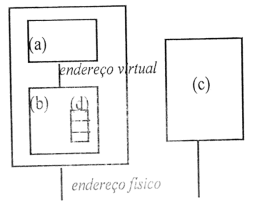
\includegraphics[width=0.4\textwidth]{ex-mem-structure}
    \end{figure}
  }

  \begin{enumerate}[label=(\alph*)]
    \item \textbf{CPU:} envia o endereço virtual à MMU;

    \item \textbf{MMU:} quebra o endereço virtual em duas partes, sendo elas a página e o deslocamento. A MMU usa $p$ como índice na TLB para obter o \textit{frame} $f$. A MMU troca a página $p$ pelo frame $f$, que é inserido no barramento junto com o deslocamento, gerando endereço físico.

    \item \textbf{Memória RAM:} entidade que contém dado desejado. Dado um endereço físico, ela acessa dado;

    \item \textbf{TLB:} é obtido o \textit{frame}, a partir do endereço virtual recebido.
  \end{enumerate}
\end{exercicio}


\begin{exercicio}
  {2º/2017}{Paginação}
  {Considere um sistema com 4 \textit{frames} e 8 páginas. Admita a seguinte \textit{string} de referência: 0172327103. Quantos \textit{page faults} ocorrerão se o algorítmo de substituição for FIFO? E se for LRU?}
  \label{ex:pagination-1}

  Fazer o exercício de forma a mostrar cada iteração e o histórico das tabelas.

  \textbf{FIFO:} 6 \textit{page faults} \\
  1ª forma:
  \[
  \begin{array}{rcccccccccc}
    \text{Página Referênciada}
    & 0 & 1 & 7 & 2 & 3 & 2 & 7 & 1 & 0 & 3 \\ \hline
    \text{Resultado}
    & P & P & P & P & P & - & - & - & P & - \\
    \\
    \text{Estado da Memória}
    & 0 & 0 & 0 & 0 & 3 & 3 & 3 & 3 & 3 & 3 \\
    & - & 1 & 1 & 1 & 1 & 1 & 1 & 1 & 0 & 0 \\
    & - & - & 7 & 7 & 7 & 7 & 7 & 7 & 7 & 7 \\
    & - & - & - & 2 & 2 & 2 & 2 & 2 & 2 & 2 \\
    \\
    \text{Ordem de saída}
    & 0 & 1 & 7 & 2 & 3 & 3 & 3 & 3 & 0 & 0 \\
    & - & 0 & 1 & 7 & 2 & 2 & 2 & 2 & 3 & 3 \\
    & - & - & 0 & 1 & 7 & 7 & 7 & 7 & 2 & 2 \\
    & - & - & - & 0 & 1 & 1 & 1 & 1 & 7 & 7 \\
  \end{array}
  \]
2ª forma:
\[
\begin{array}{rcccccccccc}
  \text{Tempo de referência}
    & 1 & 2 & 3 & 4 & 5 & 6 & 7 & 8 & 9 & 10 \\ \hline
  \text{Página Referênciada}
    & 0 & 1 & 7 & 2 & 3 & 2 & 7 & 1 & 0 & 3 \\ \hline
  \text{Resultado}
    & P & P & P & P & P & - & - & - & P & - \\
\end{array}
 \]
\begin{table}[H]
  \centering
  \begin{tabular}{lll}
    Frame & Página & Tempo de carga \\
    0     & \sout{0} 3    & \sout{1} 5            \\
    1     & \sout{1} 0    & \sout{2} 9            \\
    2     & 7             & 3              \\
    3     & 2             & 4
  \end{tabular}
\end{table}

  \textbf{LRU:} 7 \textit{page faults} \\

  1ª forma:
  \[
  \begin{array}{rcccccccccc}
    \text{Página Referênciada}
    & 0 & 1 & 7 & 2 & 3 & 2 & 7 & 1 & 0 & 3 \\ \hline
    \text{Resultado}
    & P & P & P & P & P & - & - & - & P & P \\
    \\
    \text{Estado da Memória}
    & 0 & 0 & 0 & 0 & 3 & 3 & 3 & 3 & 0 & 0 \\
    & - & 1 & 1 & 1 & 1 & 1 & 1 & 1 & 1 & 1 \\
    & - & - & 7 & 7 & 7 & 7 & 7 & 7 & 7 & 7 \\
    & - & - & - & 2 & 2 & 2 & 2 & 2 & 2 & 3 \\
    \\
    \text{Ordem de saída}
    & 0 & 1 & 7 & 2 & 3 & 2 & 7 & 1 & 0 & 3 \\
    & - & 0 & 1 & 7 & 2 & 3 & 2 & 7 & 1 & 0 \\
    & - & - & 0 & 1 & 7 & 7 & 3 & 2 & 7 & 1 \\
    & - & - & - & 0 & 1 & 1 & 1 & 3 & 2 & 7 \\
  \end{array}
  \]

2ª forma:
\[
\begin{array}{rcccccccccc}
  \text{Tempo de referência}
    & 1 & 2 & 3 & 4 & 5 & 6 & 7 & 8 & 9 & 10 \\ \hline
  \text{Página Referênciada}
    & 0 & 1 & 7 & 2 & 3 & 2 & 7 & 1 & 0 & 3 \\ \hline
  \text{Resultado}
    & P & P & P & P & P & - & - & - & P & P \\
\end{array}
 \]
\begin{table}[H]
  \centering
  \begin{tabular}{lll}
    Frame & Página                  & Tempo de referência \\
    0     & \sout{0} \sout{3} 0     & \sout{1} \sout{5} 9            \\
    1     & 1                       & \sout{2} 8            \\
    2     & 7                       & \sout{3} 7              \\
    3     & \sout{2} 3              & \sout{4} \sout{6} 10
  \end{tabular}
\end{table}

\end{exercicio}

\begin{exercicio}
  {2º/2017}{Estruturação de Sistemas Operacionais}
  {Explique a estruturação em camadas de sistema operacional. Comente vantagens e desvantagens.}

SO fica em modo protegido e seu código é distribuído em diversas camadas funcionais, de modo que rotinas de uma camada podem fazer chamadas às camadas imediatamente superior ou inferior.

 \textsc{Vantagens}:
  \begin{enumerate}
    \item Facilidade de manutenção;

    \item Modularidade;
  \end{enumerate}

 \textsc{Desvantagens}:
  \begin{enumerate}
    \item Overhead em relação ao monolítico;
  \end{enumerate}

\end{exercicio}

\begin{exercicio}
  {2º/2017}{Escalonamento de Processos}
  {Considere o conjunto de $6$ processos e respectivos tempos de execução (quantum = $4 ms$). A ordem de chegada dos processos foi $A \rightarrow B \rightarrow C \rightarrow D \rightarrow E \rightarrow F$ (do mais antigo para o mais recente). No momento de início de execução do algoritmo de escalonamento, todos os processos estão prontos. Diga a ordem na qual este conjunto será executado, considerando as políticas \textit{Round-Robin}, \textit{First Come First Served} e \textit{Shortest Job First (SJF)}.
  \begin{table}[H]
    \centering
    \begin{tabular}{cc}
      \hline \hline
      \textbf{Processo} & \textbf{Tempo de execução (ms)} \\ \hline
      A                 & 9                               \\
      B                 & 10                              \\
      C                 & 2                               \\
      D                 & 6                               \\
      E                 & 8                               \\
      E                 & 3                              \\ \hline \hline
    \end{tabular}
  \end{table}.}

  \textbf{Round-robin:} $A \rightarrow B \rightarrow C \rightarrow D \rightarrow E \rightarrow F \rightarrow A \rightarrow B \rightarrow D \rightarrow E \rightarrow A \rightarrow B$

  \textbf{SJF:} $C \rightarrow F \rightarrow D \rightarrow E \rightarrow A \rightarrow B$

  \textbf{FCFS:} $A \rightarrow B \rightarrow C \rightarrow D \rightarrow E \rightarrow F$

\end{exercicio}

\begin{exercicio}
  {2º/2017}{Organização de Sistemas Operacionais}
  {Complete o quadro abaixo com uma das seguintes características: Visão Global do Sistema, Extensibilidade, Facilidade de Manutenção de código do SO. Justifque sua resposta.
  \begin{table}[!h]
    \centering
    \begin{tabular}{clll}
      \hline \hline
      \multicolumn{1}{l}{}             & \multicolumn{1}{c}{\textbf{Monolítico}} & \multicolumn{1}{c}{\textbf{Microkernel}} & \multicolumn{1}{c}{\textbf{Exokernel}} \\ \hline
      \textbf{Visão Global do Sistema} &Alto & Médio & Baixo \\
      \hline \hline
    \end{tabular}
    \end{table}}

    \begin{itemize}
      \item Monolítico: todas as funcionalidades do SO estão no kernel;
      \item Microkernel: alguns módulos estão no modo usuário, como gerência de memória e sistema de arquivos. Porém, ele possui visão global da gerência de processos e da memória dependente do hardware;
       \item Exokernel: não conhece nenhuma abstração do SO, como gerência de processos ou sistema de arquivos. Apenas expõe o hardware e os protege;
    \end{itemize}
\end{exercicio}

\begin{exercicio}
  {2º/2017}{Arquiteturas de SO/Processos}
  {Cite os passos para a criação de processos nas arquiteturas monolíticas, \textit{microkernel} e \textit{exokernel}.}
  \label{ex:processes-creation}

  Para as \textsc{arquiteturas monolíticas}:
  \begin{enumerate}
    \item O processo pai solicita a criação de um processo filho, através de uma \textit{chamada de sistema} \texttt{create process};

    \item O SO aloca uma entrada livre na \textit{tabela de processos} para o processo filho;

    \item O SO atribui um \textit{PID} ao processo filho;

    \item O SO ajusta a \textit{área de memória} para a execução do processo filho;

    \item O SO preenche os \textit{valores de registradores} para execução do processo filho na tabela de processos;

    \item O SO insere o processo filho na fila \textit{ready} do escalonador;

    \item O SO retorna ao processo pai.
  \end{enumerate}

  Para o \textsc{microkernel}:
  \begin{enumerate}
    \item O processo pai envia uma mensagem para o microkernel, colocando o \texttt{create process} como conteúdo;

    \item O microkernel recebe a mensagem e determina que o processo filho deve ser criado;

    \item O microkernel aloca uma entrada livre na \textit{tabela de processos} para o processo filho;

    \item O microkernel atribui um \textit{PID} ao processo filho;

    \item O microkernel ajusta a \textit{área de memória} para a execução do processo filho;

    \item O microkernel preenche os \textit{valores de registradores} para execução do processo filho na tabela de processos;

    \item O microkernel insere o processo filho na fila \textit{ready} do escalonador;

    \item O microkernel envia uma mensagem para o processo pai contendo o valor de retorno.
  \end{enumerate}

  Para o \textsc{exokernel}:
  \begin{enumerate}
    \item O processo pai solicita a criação de um processo filho para a LibOS, através de uma \textit{chamada de função} \texttt{create process};

    \item A LibOS aloca uma entrada livre na \textit{tabela de processos} para o processo filho;

    \item A LibOS atribui um \textit{PID} ao processo filho;

    \item A LibOS pede uma região de software (área de memória) ao exokernel, via \textit{chamada de sistema}. Esta área é destinada ao processo filho;

    \item A LibOS solicita um \textit{processor environment} (PE), via chamada de sistema, e copiar o valor dos registradores para lá;

    \item A LibOS preenche o de prólogo e epílogo do PE (troca de contexto), descarregando o código;

    \item O exokernel coloca o PE na sua fila \textit{ready};

    \item A LibOS coloca o processo na sua fila \textit{ready};

    \item A LibOS retorna ao processo pai.
  \end{enumerate}

\end{exercicio}




\section{1º/2013}
\begin{exercicio}
  {1º/2013}{Sistemas de Arquivo}
  {Considere um arquivo de alocação contígua composto por 100 blocos, cujo tamanho máximo é 200 blocos. Quantas operações devem ser feitas caso:
  \begin{enumerate}
    \item Um bloco seja adicionado no início do arquivo.
    \item Um bloco seja adicionado no final do arquivo.
    \item Um bloco seja removido no início do arquivo.
  \end{enumerate}
  Responda o mesmo para um arquivo de mesmo tamanho que utilize lista encadeada.}

  \textbf{Para alocação contígua:}
  \begin{enumerate}
    \item 100 realocações de bloco e uma escrita, no começo;

    \item Operação de busca da posição e uma operação de escrita do bloco;

    \item Uma única operação de remoção do bloco.
  \end{enumerate}

  \textbf{Para lista encadeada:}
  \begin{enumerate}
    \item Obtenção de um bloco livre, escrita do bloco em disco e apontamento do bloco como o primeiro do arquivo, colocando o antigo primeiro bloco como o próximo;

    \item Obtenção de um bloco livre, escrita do bloco e inserção do endereço deste bloco no apontamento do antigo último bloco

    \item Remoção do bloco e apontamento do antigo segundo bloco como o novo primeiro.
  \end{enumerate}
\end{exercicio}

\begin{exercicio}
  {1º/2013}{\textit{Escalonamento de processos}}
  {Considere o conjunto de $5$ processos e respectivos tempos de execução (quantum = $8 ms$). A ordem de chegada dos processos foi $A \rightarrow B \rightarrow C \rightarrow D \rightarrow E$ (do mais antigo para o mais recente). No momento de início de execução do algoritmo de escalonamento, todos os processos estão prontos. Diga a ordem na qual este conjunto será executado, considerando as políticas \textit{Round-Robin} e \textit{Shortest Job First (SJF)}.
  \begin{table}[H]
    \centering
    \begin{tabular}{cc}
      \hline \hline
      \textbf{Processo} & \textbf{Tempo de execução (ms)} \\ \hline
      A                 & 9                               \\
      B                 & 2                              \\
      C                 & 7                               \\
      D                 & 1                               \\
      E                 & 18                              \\ \hline \hline
    \end{tabular}
  \end{table}
  } % Fim do enunciado

  Estendemos a questão, inserindo também o resultado para política FCFS. Escrevemos em ordem, do primeiro para o último:

  \textbf{Round-robin:} $A \rightarrow B \rightarrow C \rightarrow D \rightarrow E \rightarrow A \rightarrow E$

  \textbf{SJF:} $D \rightarrow B \rightarrow C \rightarrow A \rightarrow E$

  \textbf{FCFS:} $A \rightarrow B \rightarrow C \rightarrow D \rightarrow E$
\end{exercicio}

\begin{exercicio}
  {1º/2013}{\textit{Threads}}
  {Explique os $2$ níveis de implementação de threads. Cite vantagens e desvantagens.}
  \label{ex:threads-implementation-comparison}

  \textbf{\textit{Threads} a nível de usuário:} a implementação da \textit{thread} é no espaço de endereçamento do usuário, através de chamadas de funções definidas em uma biblioteca a nível de aplicação.

  \textit{Vantagens}:
  \begin{itemize}
    \item A troca de contexto entre \textit{threads} tem custo baixo, dado não é preciso de privilégio de \textit{kernel} e as estruturas compartilhadas estão a nível de usuário apenas;

    \item O escalonamento pode ser especificado dentro do processo do usuário, podendo definir-se uma política mais adequada;

    \item Caso seja implementadas por bibliotecas portáveis, podem ser executadas em qualquer SO.
  \end{itemize}

  \textit{Desvantagens:}
  \begin{itemize}
    \item Se a \textit{thread} realizar uma operação blocante, todo o processo será bloqueado até que a operação tenha resultado, bloqueando as \textit{threads-irmãs};

    \item Uma aplicação \textit{multithread} não pode tirar vantagem do multiprocessamento, já que o processo que detém as \textit{threads} apenas em um processador.
  \end{itemize}

  \textbf{\textit{Threads} a nível de \textit{kernel}:} o gerenciamento de \textit{threads} é feito pelo \textit{kernel}, manipuladas por chamadas de sistema. Cada processo contém sua tabela de \textit{threads} e o bloqueio de uma \textit{thread} não resulta no bloqueio de outras, sendo este chaveamento feito pelo \textit{kernel}.

  \textit{Vantagens:}
  \begin{itemize}
    \item Melhor aproveitamento da capacidade de multiprocessamento da máquina, escalonando várias \textit{threads} do processo em diferentes processadores;

    \item O bloqueio de uma \textit{thread} não resulta no bloqueio de outras, inclusive suas irmãs.
  \end{itemize}

  \textit{Desvantagens:}
  \begin{itemize}
    \item A troca de contexto entre \textit{threads} é custosa, uma vez que existe a passagem do modo usuário para o modo protegido.
  \end{itemize}
\end{exercicio}





\section{1º/2012}
\begin{exercicio}
  {1º/2012}{Arquiteturas de SO}
  {Admita um sistema operacional que é originalmente organizado segundo a estruturação microkernel no qual foi embutido um outro sistema operacional monolítico, por razões de desempenho. Como você classificaria esse sistema operacional? Por quê?}
\end{exercicio}

\begin{exercicio}
  {1º/2012}{Escalonamento de Processos}
  {Os escalonadores round-robin mantém, normalmente, uma fila de processos prontos, onde cada processo aparece uma só vez. Considere uma fila de prontos que mantém ponteiros para a tabela de processos. Qual seria o efeito de colocar dois ponteiros para o mesmo processo na fila de prontos $(A \rightarrow B \rightarrow C \rightarrow B)$?
  }

  O processo rodaria duas vezes por rodada, como se tivesse o dobro do quantum ou uma prioridade maior que os outros.
\end{exercicio}

\begin{exercicio}
  {1º/2012}{Escalonamento de Processos}
  {Considere o conjunto de $5$ processos e respectivos tempos de execução (quantum = $8 ms$). A ordem de chegada dos processos foi $A \rightarrow B \rightarrow C \rightarrow D \rightarrow E$ (do mais antigo para o mais recente). No momento de início de execução do algoritmo de escalonamento, todos os processos estão prontos. Diga a ordem na qual este conjunto será executado, considerando as políticas \textit{Round-Robin} e \textit{Shortest Job First (SJF)}.
  \begin{table}[h]
      \centering
      \begin{tabular}{cc}
        \hline \hline
        \textbf{Processo} & \textbf{Tempo de execução (ms)} \\ \hline
        A                 & 9                               \\
        B                 & 20                              \\
        C                 & 2                               \\
        D                 & 6                               \\
        E                 & 18                              \\
        \hline \hline
      \end{tabular}
    \end{table}
  }


    Estendemos a questão, inserindo também o resultado para política FCFS. Escrevemos em ordem, do primeiro para o último:

    \textbf{Round-robin:} $A \rightarrow B \rightarrow C \rightarrow D \rightarrow E \rightarrow A \rightarrow B \rightarrow E \rightarrow B \rightarrow E$

    \textbf{SJF:} $C \rightarrow D \rightarrow A \rightarrow E \rightarrow B$ (não tem \textit{quantum})

    \textbf{FCFS:} $A \rightarrow B \rightarrow C \rightarrow D \rightarrow E$ (não tem \textit{quantum})
\end{exercicio}

\begin{exercicio}
  {1º/2012}{Memória/Paginação}
  {Explique como funcionam as organizações \textit{forward-mapped} (mapeamento direto) e tabela invertida de páginas.}

  \textbf{Forward-mapped:} a tabela é indexada pelo endereço de página virtual, podendo existir uma entrada para cada endeço de página possível. A página indexa o \textit{frame} no qual ela deve residir na memória principal.

  \textbf{Tabela Invertida:} a tabela é indexada pelo \textit{frame}. Para obter o índice correspondente da página virtual, é aplicada uma função \textit{hash}. Como é possível haver colisões, uma entrada pode conter uma lista de colisões, contendo as páginas que coincidiram naquele \textit{frame}.
\end{exercicio}

\begin{exercicio}
  {1º/2012}{Memória/Paginação}
  {Considere um sistema com espaço de endereçamento de $32$ bits, páginas de $4$ KBytes e espaço de endereçamento real de $26$ bits.
  \begin{enumerate}[label=(\alph*)]
    \item Quantas entradas são necessárias em uma tabela de páginas forward-mapped?
    \item E na tabela de páginas invertida?
  \end{enumerate}}
\end{exercicio}

\begin{exercicio}
  {1º/2012}{Drivers}
  {O que é uma controladora? Qual entidade do SO interage com ela?}

  A controladora é a parte eletrônica das unidades de entrada e saída. Ela interage constantemente com os \textit{drivers} de dispositivo, recebendo comandos específicos de \textit{hardware} em seus registradores.
\end{exercicio}

\begin{exercicio}
  {1º/2012}{Sistemas de Arquivo}
  {Alguns sistemas de arquivo deletam todos os arquivos de usuário quando o usuário se desconecta da máquina (\textit{logoff}), a não ser que o usuário, explicitamente, diga quais arquivos devem ser permanentes. Comente esta abordagem em relação à abordagem tradicional.}

  Esta abordagem se torna interessante quando o usuário não tem o constante interesse em garantir arquivos permanentes. Também é interessante para implementações com espaço em disco rígido pequeno.
\end{exercicio}

\begin{exercicio}
  {1º/2012}{Sistemas de Arquivo}
  {Sobre \textit{buffer cache}:
  \begin{enumerate}[label=(\alph*)]
    \item Explique como as leituras e escritas em arquivos convencionais funcionam quando existe buffer cache.
    \item Explique como as leituras e escritas em arquivos convencionais funcionam quando não existe buffer cache.
  \end{enumerate}}

  \begin{enumerate}[label=(\alph*)]
    \item Quando uma operação de E/S é realizada, uma consulta a \textit{buffer cache} é realizada primeiro, onde o bloco solicitado é buscado em uma área de memória reservada. Caso não conste em memória, o bloco é buscado em disco, colocado na \textit{buffer cache} e assim efetua-se a operação.

    \item Neste caso, em todas as operações de E/S, o bloco é acessado diretamente do disco, resultando em um acesso mais lento.
  \end{enumerate}
\end{exercicio}

\begin{exercicio}
  {1º/2012}{Processos (Deadlock)}
  {Apresente uma solução para o problema do produtor-consumidor utilizando unicamente locks.}
\end{exercicio}

\begin{exercicio}
  {1º/2012}{Processos/Escalonamento}
  {O algoritmo de escalonamento de processos FCFS pode ser considerado um caso particular do algortimo Round-Robin. Qual é esse caso?}

  Quando o quantum é infinito (teoricamente). Na prática, utiliza-se o \textit{quantum} como FFFF em arquiteturas de $32$ bits e FFFF FFFF em arquiteturas de $64$ bits.
\end{exercicio}

\begin{exercicio}
  {1º/2012}{Memória/Paginação}
  {Considere a seguinte sequência de referências à páginas:
  1,2,3,4,2,1,5,6,2,1,2,3,7,6,3,2,1,2,3,6. \newline
  Quantos page faults ocorrerão para os algoritmos FCFS, ótimo e LRU, supondo que a memória real possui $4$ frames? Considere que inicialmente a memória está vazia.}

  \textbf{Nota:} use de referência a estruturação do exercício da página \pageref{ex:pagination-1}

  \textbf{FCFS:} 14 \textit{page faults} \\
  \[
  \begin{array}{cccccccccccccccccccc}
1 & 2 & 3 & 4 & 2 & 1 & 5 & 6 & 2 & 1 & 2 & 3 & 7 & 6 & 3 & 2 & 1 & 2 & 3 & 6 \\ \hline
P & P & P & P & - & - & P & P & P & P & - & P & P & P & - & P & P & - & P & - \\
\\
1 & 2 & 3 & 4 & 4 & 4 & 5 & 6 & 2 & 1 & 1 & 3 & 7 & 6 & 6 & 2 & 1 & 1 & 3 & 3 \\
- & 1 & 2 & 3 & 3 & 3 & 4 & 5 & 6 & 2 & 2 & 1 & 3 & 7 & 7 & 6 & 2 & 2 & 1 & 1 \\
- & - & 1 & 2 & 2 & 2 & 3 & 4 & 5 & 6 & 6 & 2 & 1 & 3 & 3 & 7 & 6 & 6 & 2 & 2 \\
- & - & - & 1 & 1 & 1 & 2 & 3 & 4 & 5 & 5 & 6 & 2 & 1 & 1 & 3 & 7 & 7 & 6 & 6 \\
  \end{array}
  \]

  \textbf{Ótimo:} 8 \textit{page faults}. A idéia é sempre retirar a página a ser referenciada no futuro mais distante. \\
  \[
  \begin{array}{cccccccccccccccccccc}
1 & 2 & 3 & 4 & 2 & 1 & 5 & 6 & 2 & 1 & 2 & 3 & 7 & 6 & 3 & 2 & 1 & 2 & 3 & 6 \\ \hline
P & P & P & P & - & - & P & P & - & - & - & - & P & - & - & - & P & - & - & - \\
\\
1 & 2 & 2 & 2 & 1 & 2 & 2 & 2 & 1 & 2 & 3 & 6 & 6 & 3 & 2 & 2 & 2 & 3 & 6 & 1 \\
- & 1 & 1 & 1 & 2 & 1 & 1 & 1 & 2 & 3 & 6 & 3 & 3 & 2 & 3 & 3 & 3 & 6 & 1 & 2 \\
- & - & 3 & 3 & 3 & 3 & 3 & 3 & 3 & 6 & 2 & 2 & 2 & 6 & 6 & 6 & 6 & 1 & 2 & 3 \\
- & - & - & 4 & 4 & 4 & 5 & 6 & 6 & 1 & 1 & 1 & 7 & 7 & 7 & 7 & 1 & 2 & 3 & 6 \\
  \end{array}
  \]

  \textbf{LRU:} 10 \textit{page faults} \\

\end{exercicio}

\begin{exercicio}
  {1º/2012}{Virtualização}
  {Os conceitos de \textit{full virtualization} e para \textit{virtualization} são explicados abaixo:\\
  \textit{Full Virtualization} oferece uma abstração de máquina virtual que é uma cópia exata do hardware e, portanto, permite hospedar sistemas operacionais inalterados.\\
  \textit{Virtualization} oferece uma abstração de máquina virtual que é similar, porém, não idêntica ao hardware e, por isso, requer que algumas modificações sejam feitas no sistema operacional hospedado.
  Sabendo disso, qual estrutura de sistema operacional suporta \textit{full virtualization} e qual suporta para \textit{virtualization}? Justifique sua resposta.}
\end{exercicio}

\begin{exercicio}
  {1º/2012}{Organização de Sistemas Operacionais}
  {Complete o quadro abaixo com os valores (A - Alto, M - Médio, B - Baixo). Justifque sua resposta. Atenção: Cada linha deve conter os valores Alto, Médio e Baixo.
  \begin{table}[!h]
    \centering
    \begin{tabular}{clll}
      \hline \hline
      \multicolumn{1}{l}{}             & \multicolumn{1}{c}{\textbf{Monolítico}} & \multicolumn{1}{c}{\textbf{Microkernel}} & \multicolumn{1}{c}{\textbf{Exokernel}} \\ \hline
      \textbf{Visão Global do Sistema} &&& \\
      \textbf{Extensibilidade} &&& \\
      \textbf{Flexibilidade} &&& \\
      \hline \hline
    \end{tabular}
    \caption{Tabela de comparação entre organizações}
    \label{tab:ex15}
    \end{table}}
\end{exercicio}
